\documentclass[10pt,utf8]{beamer}

\mode<presentation> {
  \usetheme{Madrid}
  \setbeamercovered{transparent}
}

\usepackage{palatino}
\usepackage{graphicx}
\usepackage{array}
\usepackage{color}
\usepackage{subfigure}
\usepackage{colortbl}
\usepackage{amsmath}
\usepackage{hyperref}
\usepackage{listings}
\usepackage{pythonhighlight} % dnf install texlive-pythonhighlight

\setbeamertemplate{caption}{\raggedright\insertcaption\par} %turn off caption prefix ("Figure")

\definecolor{delim}{RGB}{20,105,176}
\definecolor{numb}{RGB}{106, 109, 32}
\definecolor{string}{rgb}{0.64,0.08,0.08}


\title{Kafka transactions and EOS}
\author{Vojtěch Juránek}
\institute[Red Hat]{Red Hat}
\date{May 24th 2024, Debezium F2F meeting, Brno}

\newenvironment{mylisting}
{\begin{list}{}{\setlength{\leftmargin}{1em}}\item\scriptsize\bfseries}
{\end{list}}

\newenvironment{mytinylisting}
{\begin{list}{}{\setlength{\leftmargin}{1em}}\item\tiny\bfseries}
{\end{list}}


\begin{document}

%\tikzstyle{every picture}+=[remember picture]
%\tikzstyle{na} = [baseline=-.5ex]


\begin{frame}
    \titlepage
\end{frame}

\begin{frame}
    \begin{itemize}
        \item Idempotent producers.
        \item Transactions 
        \item Exactly once semantics.
    \end{itemize}
\end{frame}

\begin{frame}
    \frametitle{Idempotent producer}
    \begin{itemize}
        \item Each producer has assigned unique ID (PID) and epoch/generation.
        \item Each message has assigned sequence number that is incremented for every message sent.
        \item Broker keep maximum sequence number for given producer and partition (high watermark).
        \item Message is accepted by the broken only when the sequence number of the message for given epoch is high watermark + 1.
    \end{itemize}
\end{frame}

\begin{frame}
    \frametitle{Kafka transactions}
    \begin{itemize}
        \item Atomic writes across multiple Kafka topics and partitions.
        \item Atomic read-process-write cycles.
        \item Producer can run at most one ongoing transaction.
        \item Consumer delivers transactional messages to the application only if the transaction was committed.
        \item However, consumer is not guaranteed to be subscribed to all partitions that are part of the transaction.
    \end{itemize}
\end{frame}

\begin{frame}
    \frametitle{Transaction coordinator}
    \begin{itemize}
        \item Runs inside every Kafka broker.
        \item Takes care about transaction log - an internal Kafka topic, more specifically is a leader of selected partitions of transaction log.
        \item Transaction log stores only state of the transaction and associated metadata, not the records themselves.
        \item Owns subset of partitions in transaction log - for these partitions for which broker is the leader.
    \end{itemize}
\end{frame}

\begin{frame}
    \frametitle{Transaction coordinator}
    \begin{figure}
        \centering
        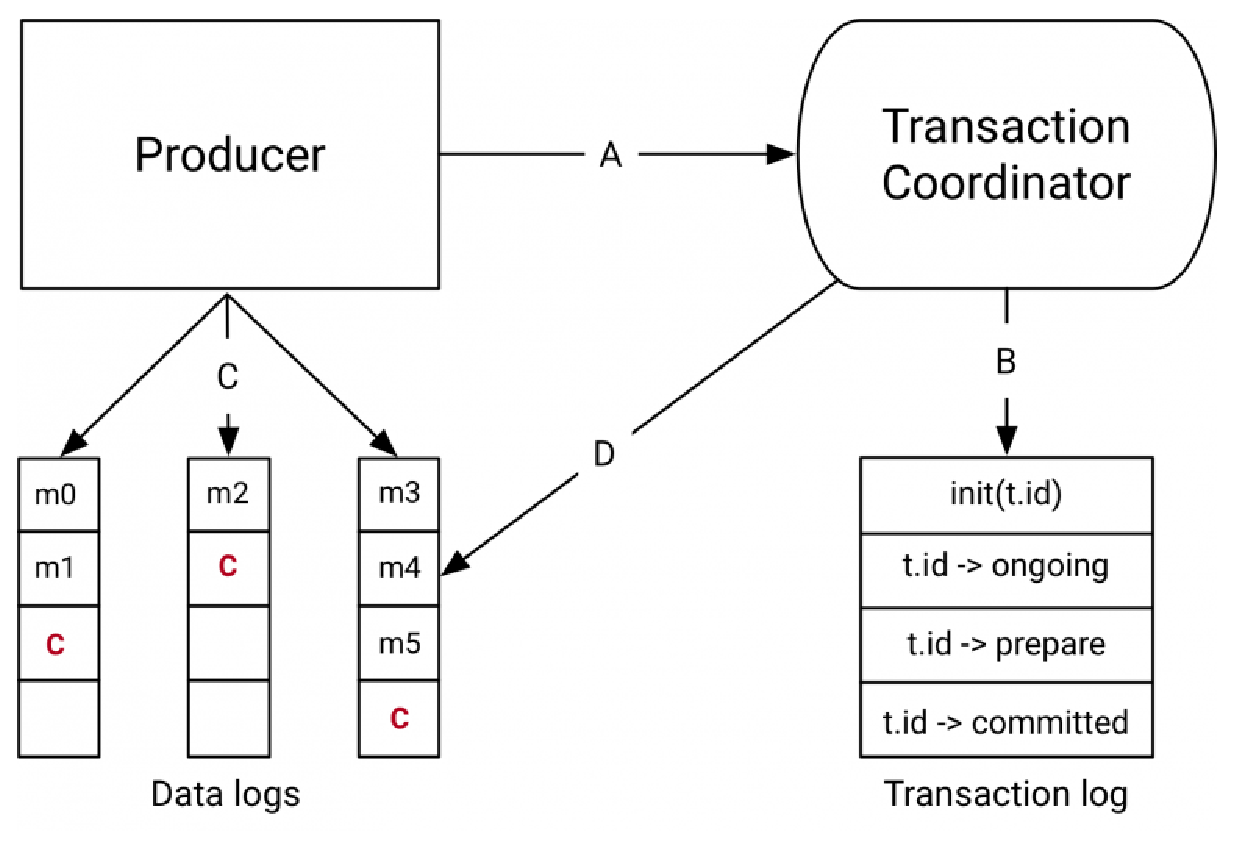
\includegraphics[height=6cm]{./img/kafka_transactions.eps}
        \caption{\tiny{Source: \url{https://www.confluent.io/blog/transactions-apache-kafka/}}}
    \end{figure}
\end{frame}

\begin{frame}
    \frametitle{Transaction flow}
    \begin{enumerate}
        \item Producer finds transaction coordinator for its group.
    \end{enumerate}
    \begin{figure}
        \centering
        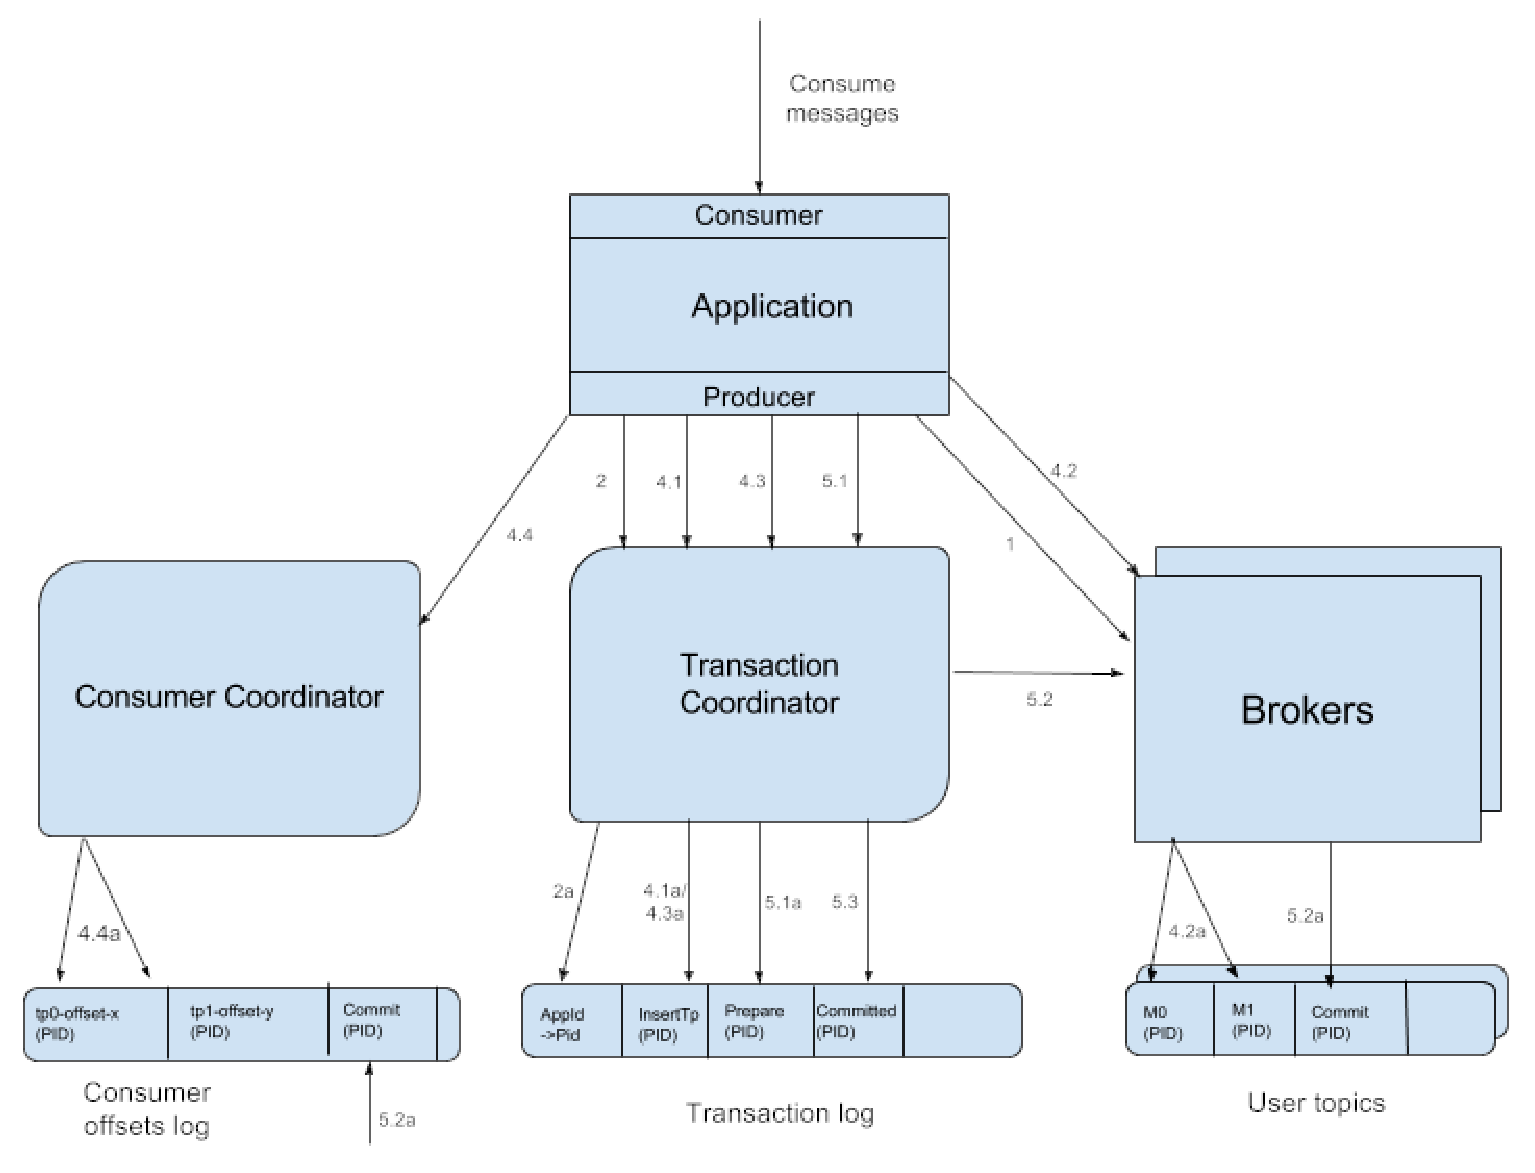
\includegraphics[height=6cm]{./img/tx_flow.eps}
        \caption{\tiny{Source: \url{https://cwiki.apache.org/confluence/display/KAFKA/KIP-98+-+Exactly+Once+Delivery+and+Transactional+Messaging}}}
    \end{figure}
\end{frame}

\begin{frame}
    \frametitle{Transaction flow}
    \begin{enumerate}
        \setcounter{enumi}{1}
        \item Producer obtains producer ID (PID).
        \begin{itemize}
          \item Based on it's \texttt{transactional.id} producer obtains PID from the coordinator.
          \item Coordinator also bumps the epoch for given producer
          \item and resolves exiting pending transaction from given producer 
        \end{itemize}
    \end{enumerate}
    \begin{figure}
        \centering
        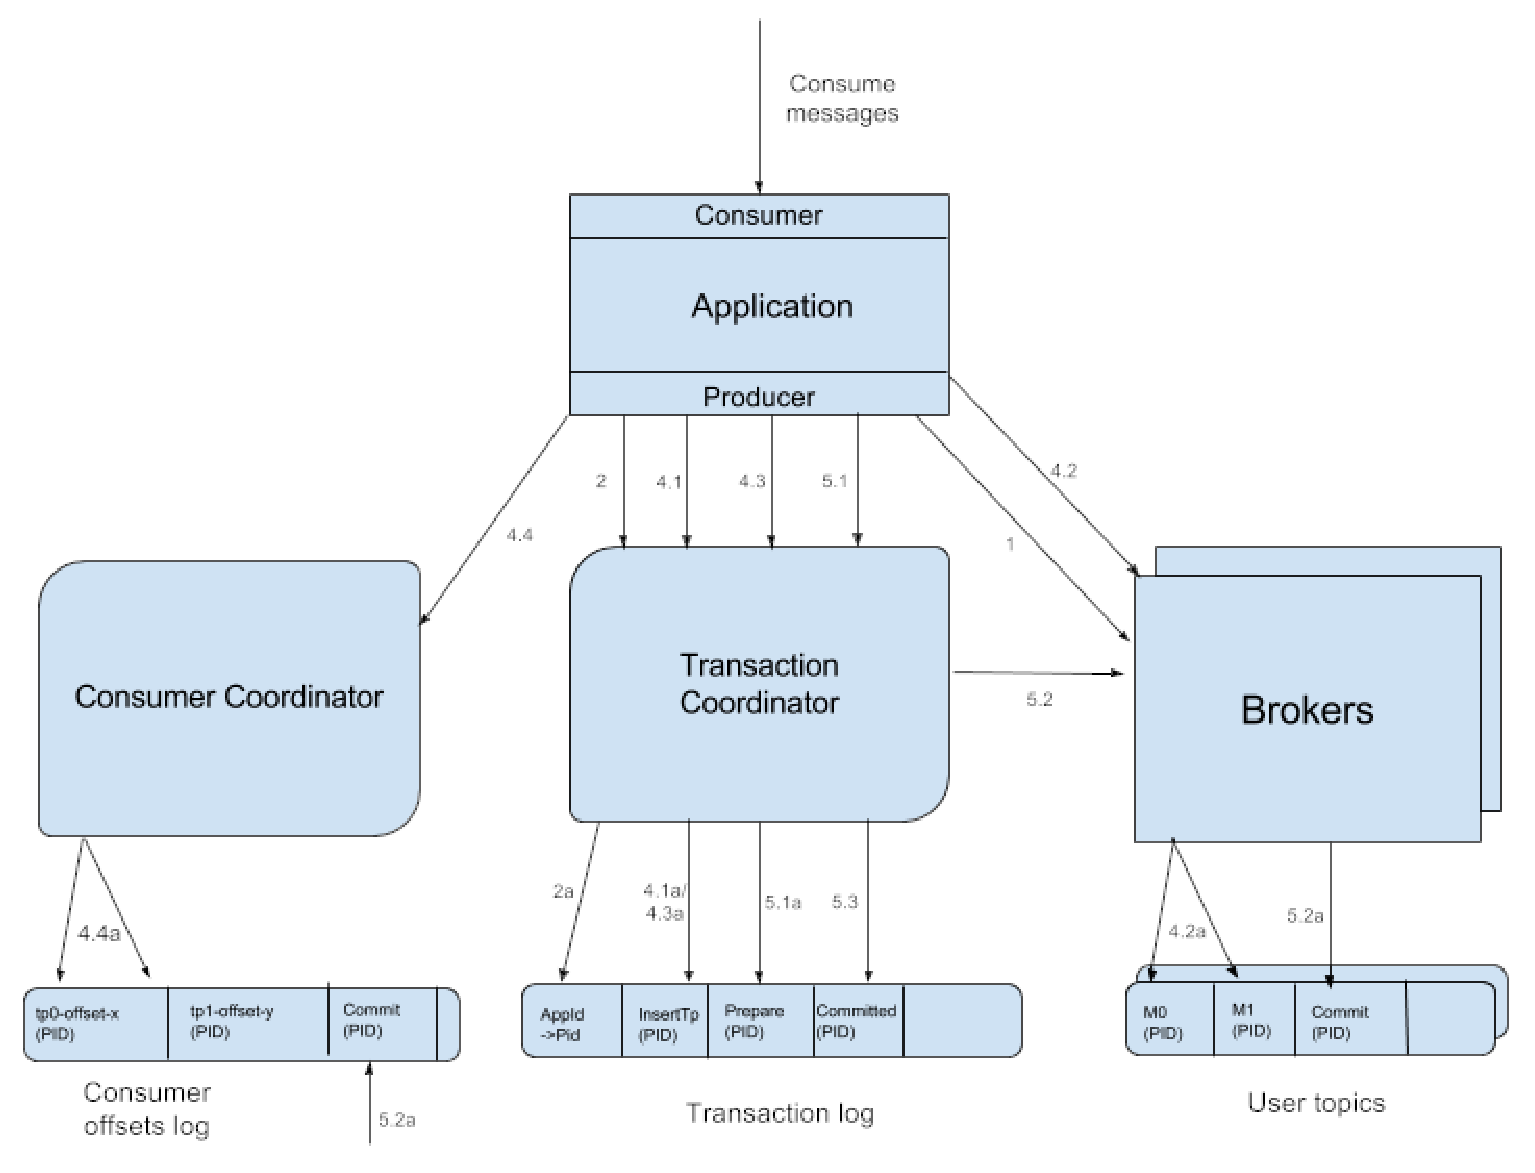
\includegraphics[height=6cm]{./img/tx_flow.eps}
        \caption{\tiny{Source: \url{https://cwiki.apache.org/confluence/display/KAFKA/KIP-98++Exactly+Once+Delivery+and+Transactional+Messaging}}}
    \end{figure}
\end{frame}

\begin{frame}
    \frametitle{Transaction flow}
    \begin{enumerate}
        \setcounter{enumi}{2}
        \item Producer starts the transaction (calls \texttt{beginTransaction()}).
    \end{enumerate}
    \begin{figure}
        \centering
        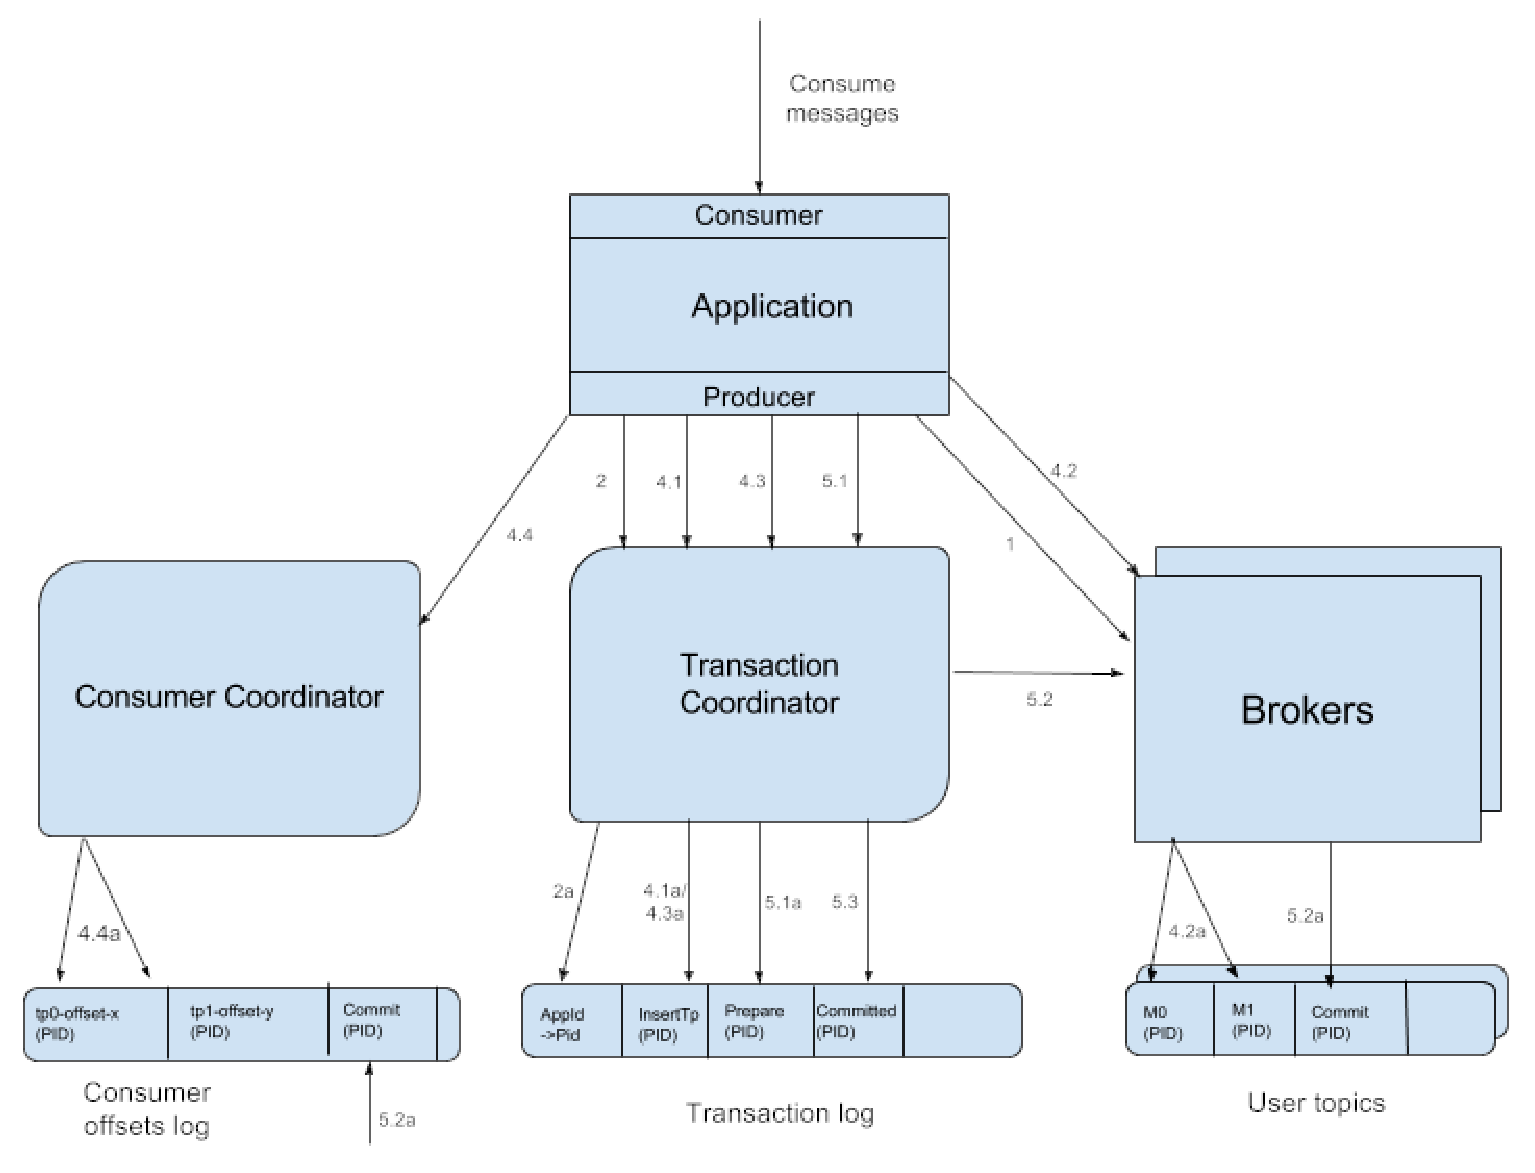
\includegraphics[height=6cm]{./img/tx_flow.eps}
        \caption{\tiny{Source: \url{https://cwiki.apache.org/confluence/display/KAFKA/KIP-98++Exactly+Once+Delivery+and+Transactional+Messaging}}}
    \end{figure}
\end{frame}

\begin{frame}
    \frametitle{Transaction flow}
    \begin{enumerate}
        \setcounter{enumi}{3}
        \item Consume-transform-produce loop.
          \begin{itemize}
            \item Producer requests adding partitions to TX request.
            \item Coordinator starts TX timer.
            \item Producer sends TX messages.
            \item Producer sends TX coordinator request for adding offsets into TX (enables batching of consumer and produced messages).
            \item Producer sends TX offset commit request to the consumer coordinator.
          \end{itemize}
    \end{enumerate}
    \begin{figure}
        \centering
        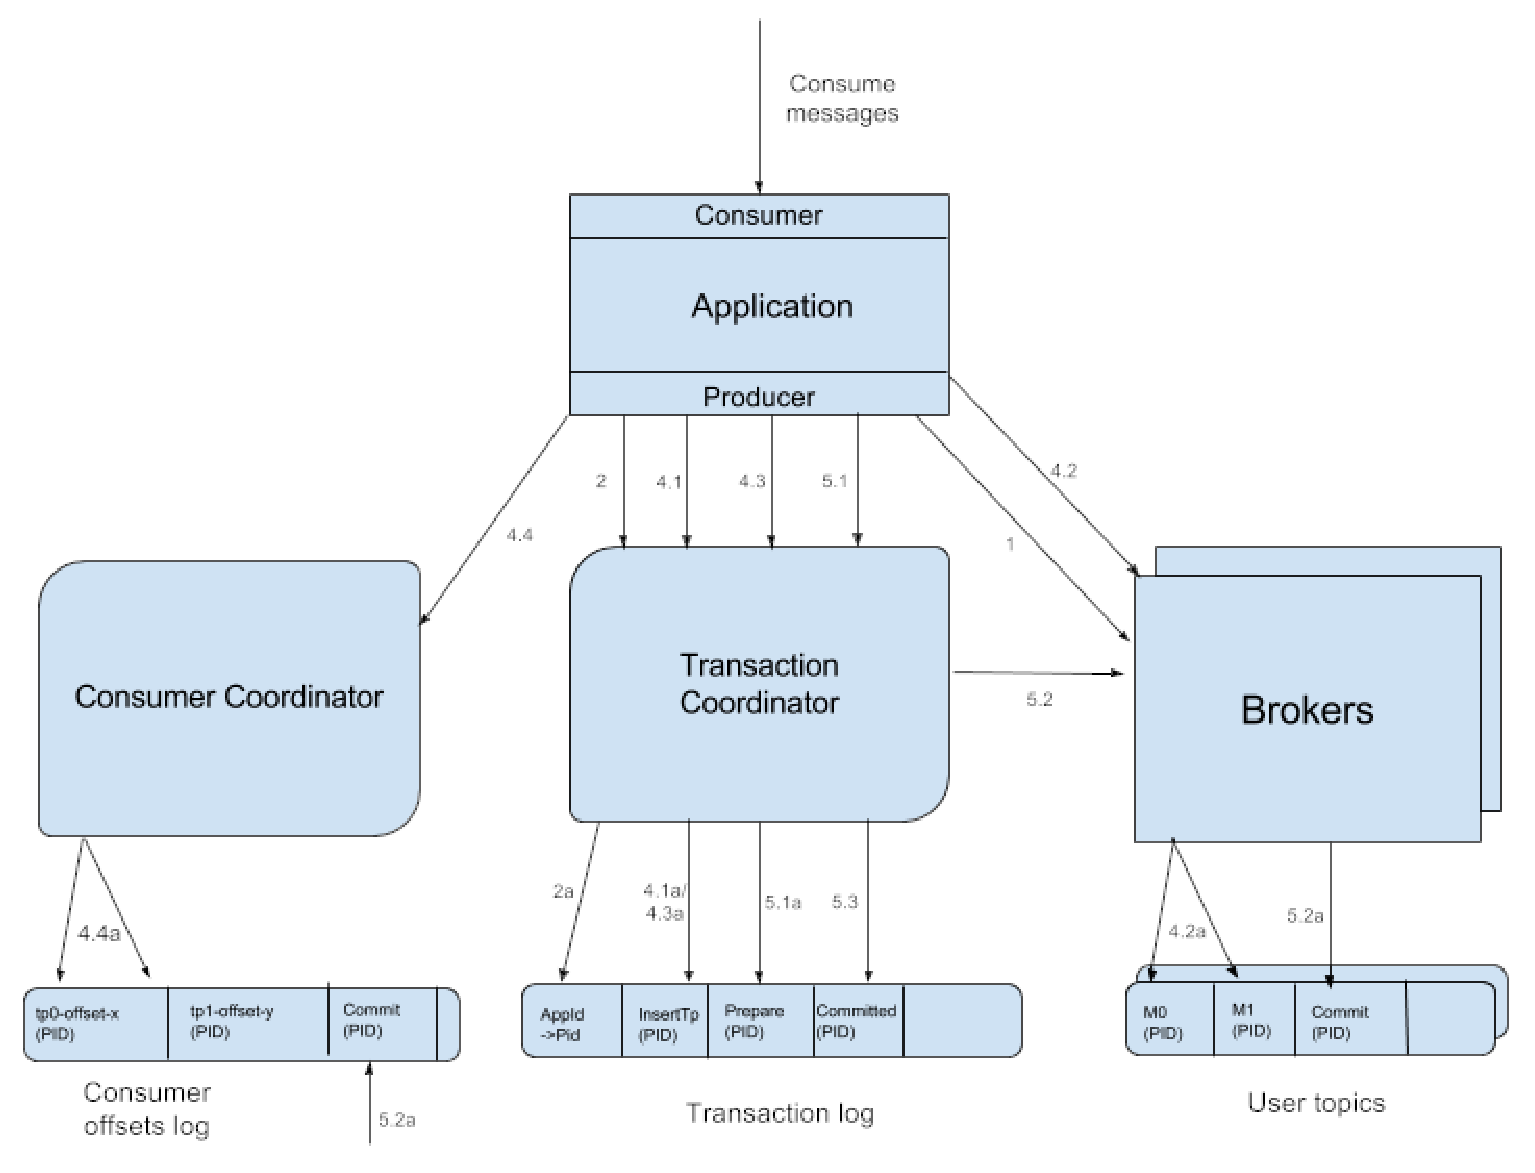
\includegraphics[height=5cm]{./img/tx_flow.eps}
        \caption{\tiny{Source: \url{https://cwiki.apache.org/confluence/display/KAFKA/KIP-98++Exactly+Once+Delivery+and+Transactional+Messaging}}}
    \end{figure}
\end{frame}

\begin{frame}
    \frametitle{Transaction flow}
    \begin{enumerate}
        \setcounter{enumi}{4}
        \item Transaction is committed or aborted.
        \begin{itemize}
          \item Coordinator writes prepare commit or prepare abort to TX log.
          \item Coordinator sends commit to user logs.
          \item Coordinator writes \texttt{commit} to TX log.
          \item Coordinator sends TX marker to partition leaders of affected partitions.
          \item Partitions leaders \texttt{commit} to their logs.
          \item Coordinator writes \texttt{committed} to TX log.
          \item Consumers delivers TX messages.
        \end{itemize}
    \end{enumerate}
    \begin{figure}
        \centering
        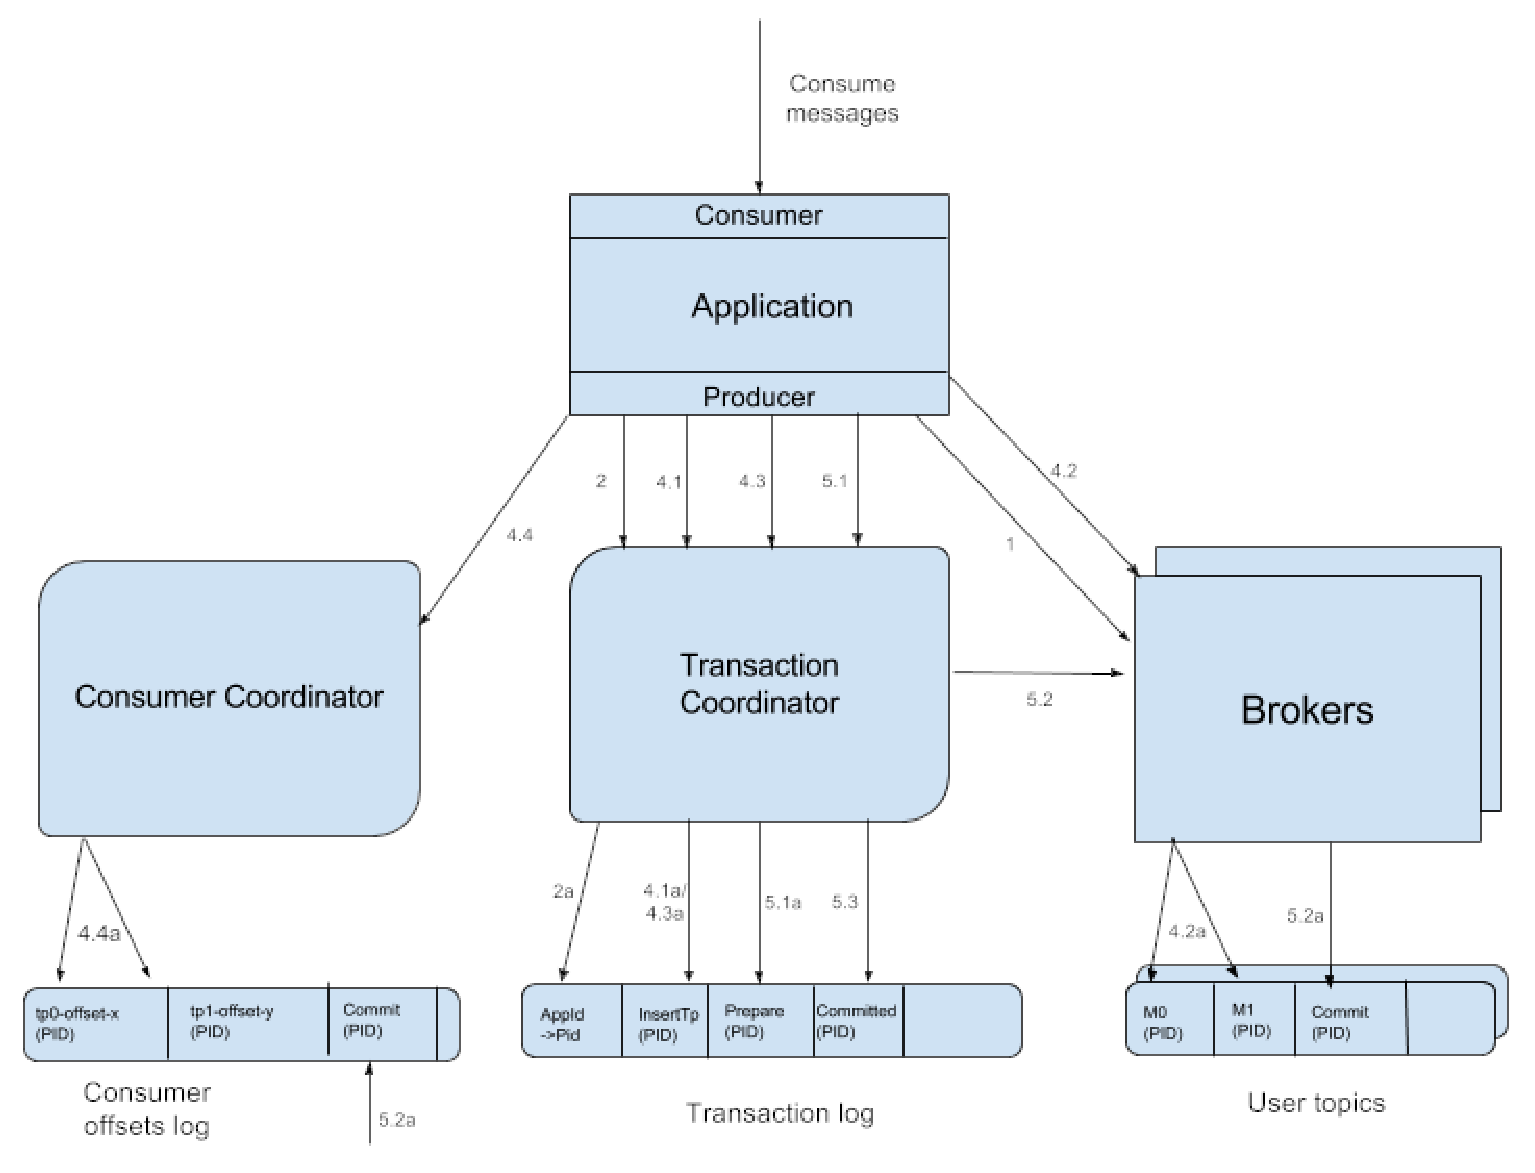
\includegraphics[height=5cm]{./img/tx_flow.eps}
        \caption{\tiny{Source: \url{https://cwiki.apache.org/confluence/display/KAFKA/KIP-98++Exactly+Once+Delivery+and+Transactional+Messaging}}}
    \end{figure}
\end{frame}

% \begin{frame}
%     \frametitle{Transaction flow}
%     \begin{enumerate}
%         \item Producer finds transaction coordinator for its group.
%         \item Producer obtains producer ID (PID).
%         \begin{itemize}
%           \item Based on it's \texttt{transactional.id} producer obtains PID from the coordinator.
%           \item also bumps the epoch for given producer
%           \item and resolves exiting pending transaction from given producer 
%         \end{itemize}
%         \item Producer starts the transaction (calls \texttt{beginTransaction()}).
%         \item Consume-transform-produce loop.
%           \begin{itemize}
%             \item Coordinator starts TX timer.
%             \item Producer requests adding partitions to TX request.
%             \item Producer sends TX messages.
%             \item Producer sends request for adding offsets into TX (enables batching of consumer and produced messages).
%             \item Producer sends TX offset commit request to the coordinator.
%           \end{itemize}
%         \item Transaction is committed or aborted.
%         \begin{itemize}
%           \item Coordinator writes prepare commit or prepare abort to TX log.
%           \item Coordinator sends commit to user logs.
%           \item Coordinator writes \texttt{commit} to TX log.
%           \item Coordinator sends TX marker to partition leaders of affected partitions.
%           \item Partitions leaders \texttt{commit} to their logs.
%           \item Coordinator writes \texttt{committed} to TX log.
%           \item Consumers delivers TX messages.
%         \end{itemize}
%     \end{enumerate}
% \end{frame}
% 
% \begin{frame}
%     \frametitle{Transaction flow}
%     \begin{figure}
%         \centering
%         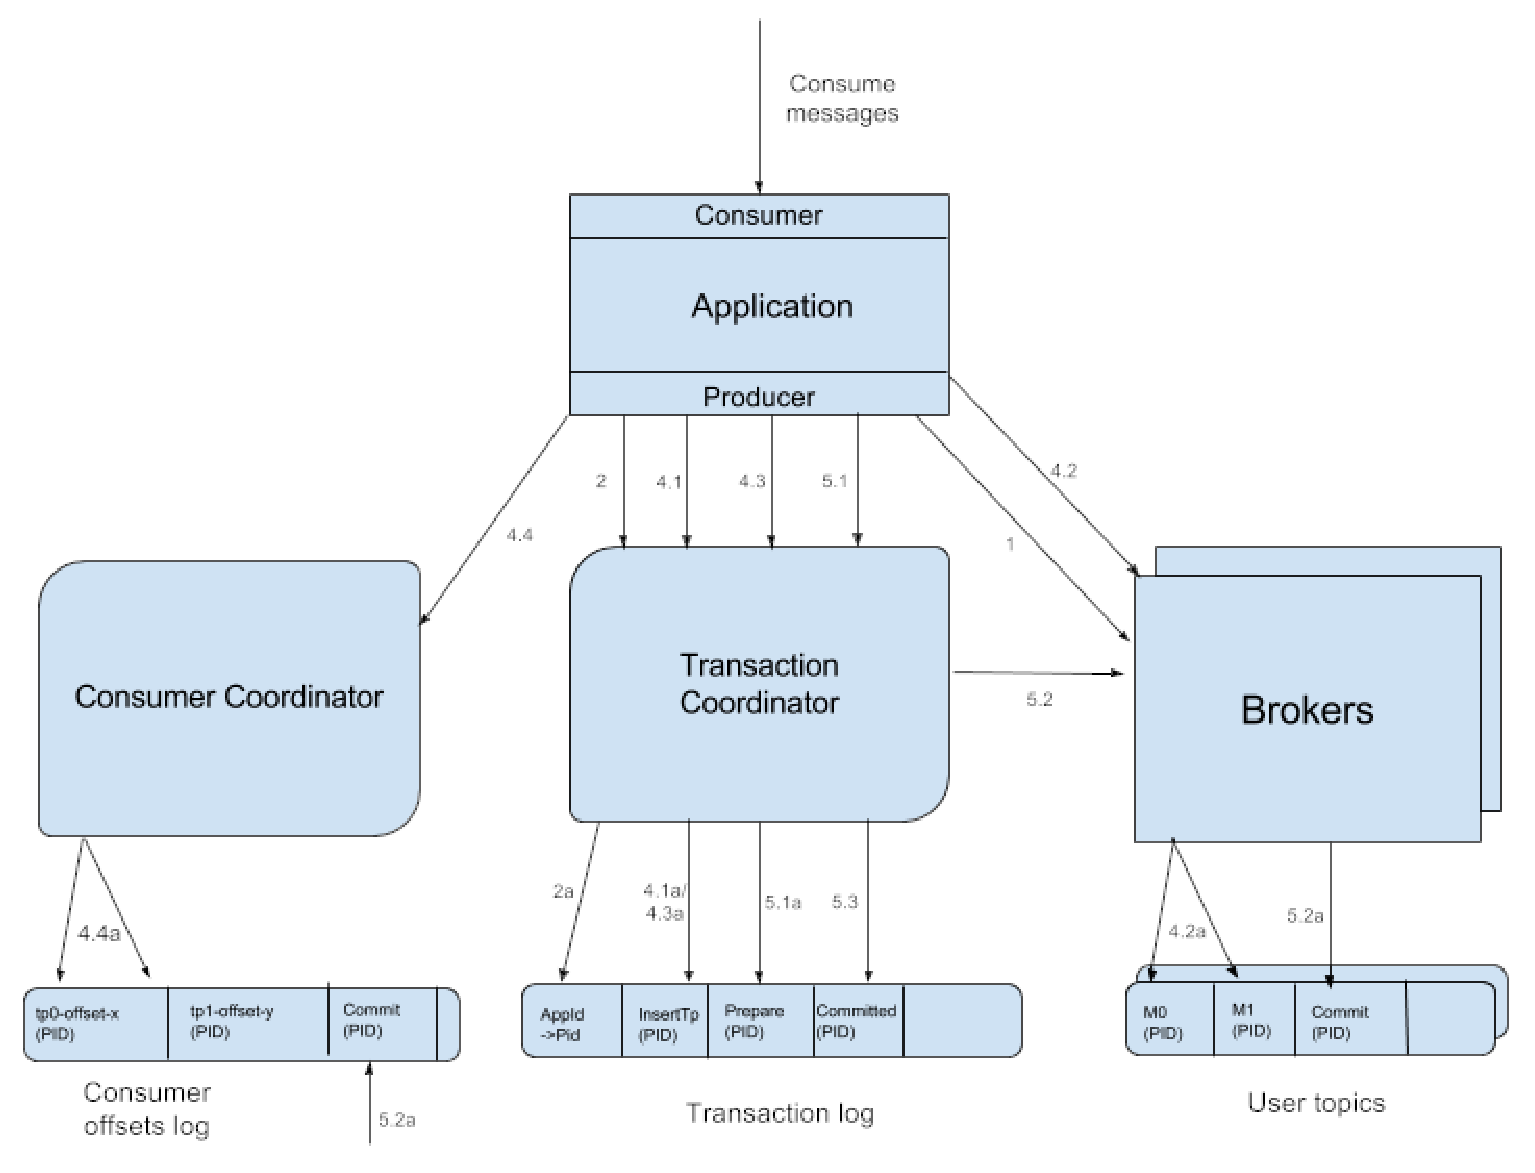
\includegraphics[height=7cm]{./img/tx_flow.eps}
%         \caption{\tiny{Source: \url{https://cwiki.apache.org/confluence/display/KAFKA/KIP-98+-+Exactly+Once+Delivery+and+Transactional+Messaging}}}
%     \end{figure}
% \end{frame}

\begin{frame}
    \frametitle{Offsets}
    \begin{itemize}
      \item Last stable offset (LSO) - all lower offsets have been decided (committed or aborted).
      \item First unstable offset (FUO) - the earliest offset that is part of the ongoing transaction.
      \item High watermark (HW) - the offset of the last message that was successfully copied to all of the log’s in-sync replicas.
      \item Log end offset (LEO) - the the highest offset of the partition.
    \end{itemize}

    \begin{figure}
        \centering
        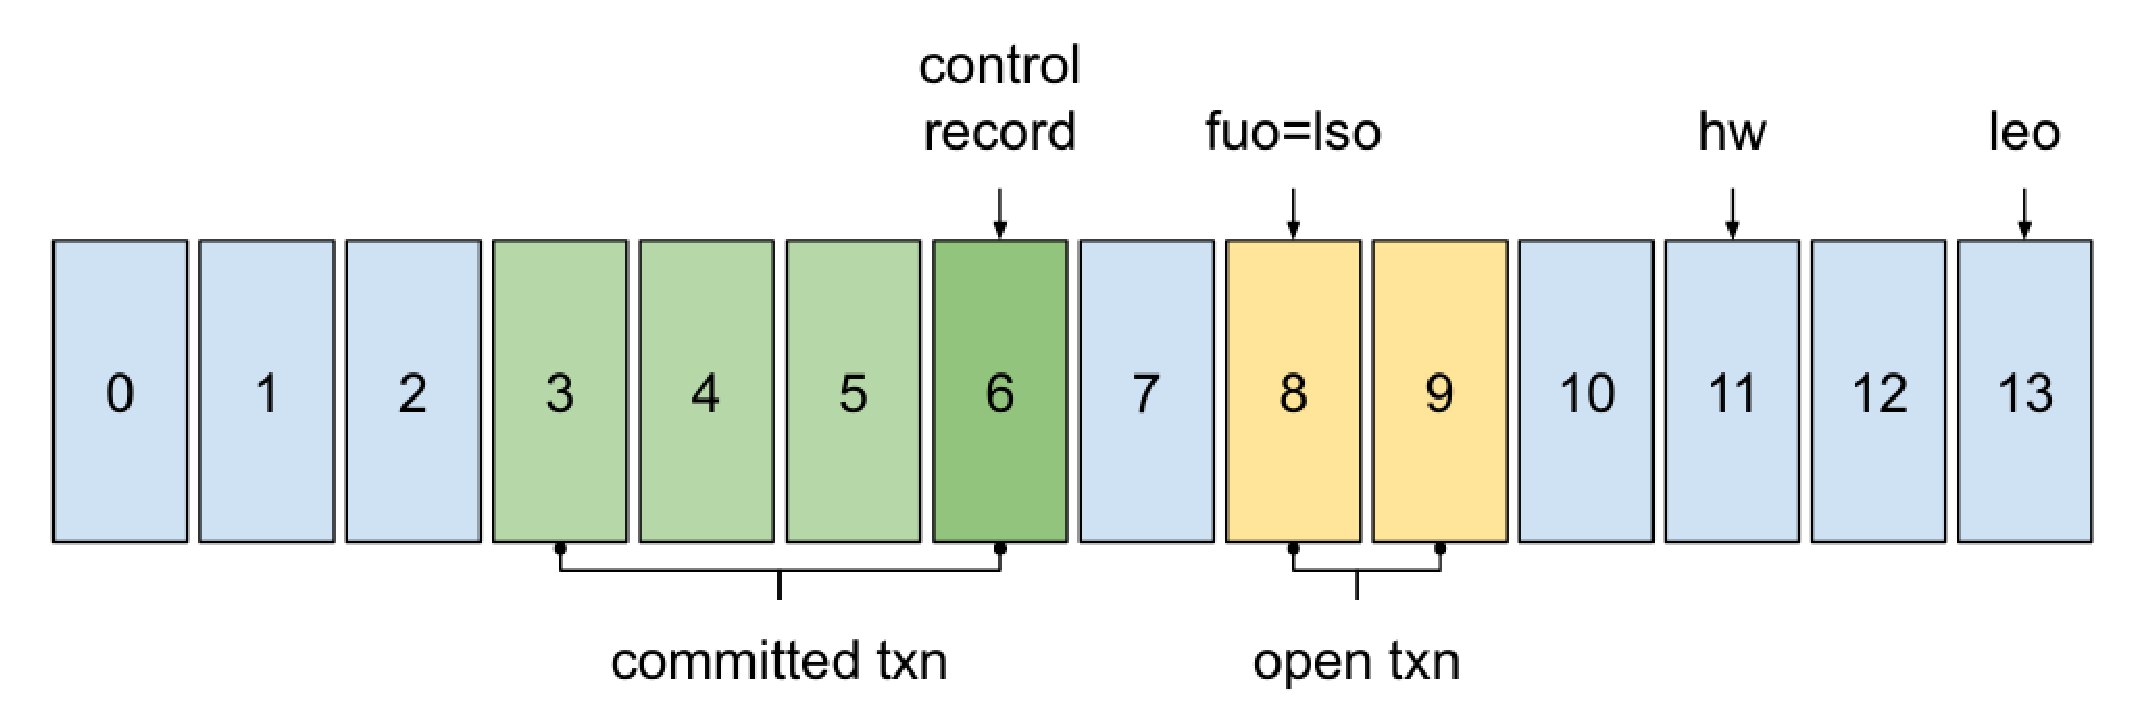
\includegraphics[height=4cm]{./img/tx_offsets.eps}
        \caption{\tiny{Source: \url{https://strimzi.io/blog/2023/05/03/kafka-transactions/}}}
    \end{figure}
\end{frame}

\begin{frame}
    \frametitle{Related config options}
    Producer config:
    \begin{itemize}
        \item \texttt{enable.idempotence} - must be set to \texttt{true}.
        \item \texttt{transaction.timeout.ms} - maximum amout of time the coordinator will wait for transaction to be completed.
        \item \texttt{transactional.id} - has to be unique per producer.
    \end{itemize}
    
    \vspace{0.5cm}
    
    Consumer config:
    \begin{itemize}
     \item \texttt{isolation.level = read\_uncommitted | read\_committed}
    \end{itemize}
    
    \vspace{0.5cm}
    
    Broker config - has the sane defaults
    \begin{itemize}
      \item \texttt{transactional.id.timeout.ms}
      \item \texttt{max.transaction.timeout.ms}
      \item \texttt{transaction.state.log.replication.factor}
      \item \texttt{transaction.state.log.num.partitions}
      \item \texttt{transaction.state.log.min.isr}
      \item \texttt{transaction.state.log.segment.bytes}
    \end{itemize}
\end{frame}

\begin{frame}
    \frametitle{KIP-618: Source connector EOS}
    \begin{itemize}
      \item Wraps everything (sending records, committing offsets) into a transaction.
      \item Kafka TX framework also fences zombie producers.
      \item Source connector has to be able to resume from it's (external resource) offset position.
    \end{itemize}
\end{frame}

\begin{frame}
    \frametitle{Source connector EOS related config options}
    Worker config:
    \begin{itemize}
        \item \texttt{exactly.once.source.support = disabled | preparing | enabled}
    \end{itemize}
    
    \vspace{0.5cm}
    
    Consumer config:
    \begin{itemize}
     \item \texttt{exactly.once.support = requested | required}
     \item \texttt{transaction.boundary = poll | interval | connector}
     \item \texttt{offsets.storage.topic}
     \item \texttt{transaction.boundary.interval.ms}
    \end{itemize}
\end{frame}

\begin{frame}
    \frametitle{Resource}
    \begin{itemize}
        \color{blue}
        \item \href{https://cwiki.apache.org/confluence/display/KAFKA/Idempotent+Producer}{Kafka Idempotent Producer}
        \item \href{https://cwiki.apache.org/confluence/display/KAFKA/Transactional+Messaging+in+Kafka}{Kafka Transactional Messaging}
        \item \href{https://cwiki.apache.org/confluence/display/KAFKA/KIP-98+-+Exactly+Once+Delivery+and+Transactional+Messaging}{Kafka KIP-98: Exactly Once Delivery and Transactional Messaging}
        \item \href{https://cwiki.apache.org/confluence/display/KAFKA/KIP-618\%3A+Exactly-Once+Support+for+Source+Connectors}{Kafka KIP-618: Exactly-Once Support for Source Connectors}
        \item \href{https://docs.google.com/document/d/11Jqy\_GjUGtdXJK94XGsEIK7CP1SnQGdp2eF0wSw9ra8/edit\#heading=h.xq0ee1vnpz4o}{Exactly Once Delivery and Transactional Messaging in Kafka (design document)}
        \item \href{https://www.confluent.io/blog/transactions-apache-kafka/}{Transactions in Apache Kafka (Confluent blog)}
        \item \href{https://strimzi.io/blog/2023/05/03/kafka-transactions/}{Exactly-once semantics with Kafka transactions (Strimzi blog)}
        \color{black}
    \end{itemize}
\end{frame}

\begin{frame}
    \frametitle{Questions?}
    \centering
     \textbf{\Huge{Thank you!}}
    
    \vspace{1.5cm}
    
    \textbf{\Huge{Questions?}}
    
    \vspace{1cm}
\end{frame}

%%%%%%%%%%%%%%%%%%%%%%%%%%%%%%%%%%%%%%%%%%%%%%%%%%%%%%%%%%%%%%%%%%%%%%%%%%%%%%%%%%%%%%%%%%%%%%%%%
%%% BACKUP
%%%%%%%%%%%%%%%%%%%%%%%%%%%%%%%%%%%%%%%%%%%%%%%%%%%%%%%%%%%%%%%%%%%%%%%%%%%%%%%%%%%%%%%%%%%%%%%%%

% \begin{frame}
%     \centering
%     \huge{\textbf{Backup slides}}
% \end{frame}

\end{document}
